\documentclass[12pt,]{article}
\usepackage[left=1in,top=1in,right=1in,bottom=1in]{geometry}
\newcommand*{\authorfont}{\fontfamily{phv}\selectfont}
\usepackage[]{mathpazo}


  \usepackage[T1]{fontenc}
  \usepackage[utf8]{inputenc}




\usepackage{abstract}
\renewcommand{\abstractname}{}    % clear the title
\renewcommand{\absnamepos}{empty} % originally center

\renewenvironment{abstract}
 {{%
    \setlength{\leftmargin}{0mm}
    \setlength{\rightmargin}{\leftmargin}%
  }%
  \relax}
 {\endlist}

\makeatletter
\def\@maketitle{%
  \newpage
%  \null
%  \vskip 2em%
%  \begin{center}%
  \let \footnote \thanks
    {\fontsize{18}{20}\selectfont\raggedright  \setlength{\parindent}{0pt} \@title \par}%
}
%\fi
\makeatother




\setcounter{secnumdepth}{0}

\usepackage{longtable,booktabs}



\title{Predicting Opinion Change in Deliberative Groups (Natural Language
Processing) \thanks{Code and data available at: github.com/rossdahlke/cs\_230\_project}  }



\author{\Large Ross Dahlke
(\href{mailto:rdahlke@stanford.edu}{\nolinkurl{rdahlke@stanford.edu}})\vspace{0.05in} \newline\normalsize\emph{}  }


\date{}

\usepackage{titlesec}

\titleformat*{\section}{\normalsize\bfseries}
\titleformat*{\subsection}{\normalsize\itshape}
\titleformat*{\subsubsection}{\normalsize\itshape}
\titleformat*{\paragraph}{\normalsize\itshape}
\titleformat*{\subparagraph}{\normalsize\itshape}





\newtheorem{hypothesis}{Hypothesis}
\usepackage{setspace}


% set default figure placement to htbp
\makeatletter
\def\fps@figure{htbp}
\makeatother

\usepackage{graphicx}

% move the hyperref stuff down here, after header-includes, to allow for - \usepackage{hyperref}

\makeatletter
\@ifpackageloaded{hyperref}{}{%
\ifxetex
  \PassOptionsToPackage{hyphens}{url}\usepackage[setpagesize=false, % page size defined by xetex
              unicode=false, % unicode breaks when used with xetex
              xetex]{hyperref}
\else
  \PassOptionsToPackage{hyphens}{url}\usepackage[draft,unicode=true]{hyperref}
\fi
}

\@ifpackageloaded{color}{
    \PassOptionsToPackage{usenames,dvipsnames}{color}
}{%
    \usepackage[usenames,dvipsnames]{color}
}
\makeatother
\hypersetup{breaklinks=true,
            bookmarks=true,
            pdfauthor={Ross Dahlke
(\href{mailto:rdahlke@stanford.edu}{\nolinkurl{rdahlke@stanford.edu}}) ()},
             pdfkeywords = {},  
            pdftitle={Predicting Opinion Change in Deliberative Groups (Natural Language
Processing)},
            colorlinks=true,
            citecolor=blue,
            urlcolor=blue,
            linkcolor=magenta,
            pdfborder={0 0 0}}
\urlstyle{same}  % don't use monospace font for urls

% Add an option for endnotes. -----


% add tightlist ----------
\providecommand{\tightlist}{%
\setlength{\itemsep}{0pt}\setlength{\parskip}{0pt}}

% add some other packages ----------

% \usepackage{multicol}
% This should regulate where figures float
% See: https://tex.stackexchange.com/questions/2275/keeping-tables-figures-close-to-where-they-are-mentioned
\usepackage[section]{placeins}


\begin{document}
	
% \pagenumbering{arabic}% resets `page` counter to 1 
%
% \maketitle

{% \usefont{T1}{pnc}{m}{n}
\setlength{\parindent}{0pt}
\thispagestyle{plain}
{\fontsize{18}{20}\selectfont\raggedright 
\maketitle  % title \par  

}

{
   \vskip 13.5pt\relax \normalsize\fontsize{11}{12} 
\textbf{\authorfont Ross Dahlke
(\href{mailto:rdahlke@stanford.edu}{\nolinkurl{rdahlke@stanford.edu}})} \hskip 15pt \emph{\small }   

}

}






\vskip -8.5pt


 % removetitleabstract

\noindent \singlespacing 

\hypertarget{introduction}{%
\section{1. Introduction}\label{introduction}}

Deliberative Democracy is when a representative sample of people come
together for a short period of time to discuss civic issues. The idea is
that through a deliberative process, where people have access to
objective information and good conditions to discuss, people can come to
conclusions on civic issues that are most representative of what people
actually want (Fishkin 2018). In a time where so much discussion about
political and civic issues happens in online information bubbles,
Deliberative Democracy offers a chance for people to discuss issues on
their merit and the freedom to change their opinions in order to reveal
a better representation of public opinion.

Deliberative Democracy Polling is a technique pioneered by Stanford
University Professor Jim Fishkin and the Center for Deliberative
Democracy (CDD). A Deliberative Poll is where individuals are asked
about their opinions before and after a weekend of small-group
deliberation. This method allows researchers to measure the change in
people's opinions as a result of the deliberative sessions.

For example, one session in Ghana was about water and agricultural
policies in the country. Here is a excerpt of one of the participants
expressing their opinion to the group when talking about farmers and
their personal beliefs.

\begin{quote}
What would really help our farmers is the marketing of their produce.
That is what the farmers need. If they aren't able to better market
their produce, you would see that middlemen come and take advantage of
them. At the end of the day, the farmers are frustrated and have to sell
for less. This isn't a good thing and needs to be addressed to support
our farmers. The government needs to do this. In the past, we had food
distribution companies, rice mills and others that used to buy from the
farmers. That isn't there anymore. This would make the farmers happy and
encourage them to farm more. But if they always have to sell and run
losses, it is very frustrating for them.
\end{quote}

\hypertarget{related-work}{%
\section{2. Related work}\label{related-work}}

This project derives its inspiration from two main papers: ``Attitude
Change on Reddit's Change My View'' (Priniski and Horne 2018) and ``A
Deep-Learning Approach for Identifying Collective Action Events with
Text and Image Data from Social Media'' (Zhang and Pan 2019). The former
paper found that the ``the amount of evidence provided in a discussion
predicts attitude change'' on the Change My View Reddit forum. The
latter paper was able to identify collective action events in China
based on image and text data and provides inspiration on using text data
to identify collective behavior that has real-world application and can
be a component of future computational social science research.

\hypertarget{dataset-and-features}{%
\section{3. Dataset and Features}\label{dataset-and-features}}

This project thanks the CDD for sharing their data. For this project, I
have access to surveys and transcripts from three Deliberative Polls,
each consisting of about 14 groups, with each group discussing in two or
three different sessions. The surveys allow me to calculate opinion
change on the issues discussed in each session before and after the
deliberations. I use these pre- and post-surveys (responses on a 1-10
scale) to calculate an average delta in opinion change for each
deliberative group for each topic session which I use as my dependent
variable.\footnote{See
  \url{https://github.com/rossdahlke/cs_230_project/blob/master/preanalysis/preanalysis.pdf}
  for a pre-analysis of the distribution of survey data} The transcripts
are broken down by group by session, but they are not attributed to
specific individuals. While the additional granularity of
individually-attributed transcripts would have great and is something to
consider devoting resources to in the future, these group-level opinion
deltas and transcripts provide enough data to complete the task. In
total, there are 101 examples.

\hypertarget{methods}{%
\section{4. Methods}\label{methods}}

To capture changes in the differences in the words that discussants use
through their deliberations, I break each transcript down into 1/10th
chunks. I then calculated the similarity of each 1/10th chunk to each
other by comparing the word embeddings of each chunk. I used
similarities from the spacy core model (Honnibal and Montani 2017) and
BERT {[}citation. For example, of a given transcript, there might be a
similarity of .9 between the first and second 1/10th chunks and a
similarity of .7 between the third and fourth 1/10th chunks. I use these
similarities from each transcript to build two simple OLS models
(Pedregosa et al. 2011). The first baseline model just uses the
similarity of the second and tenth chunks (the first chunk is generally
devoted to introductions, welcomes, etc.) to predict opinion deltas. The
second model uses all of the similarities to try to predict opinion
deltas. I also train a basic neural network in Pytorch (Paszke et al.
2019) to try to predict the opinion deltas from all of the similarities.
The BERT embeddings performed better than the spacy core model in the
regressions, but not in the basic neural network.

\begin{figure}

{\centering 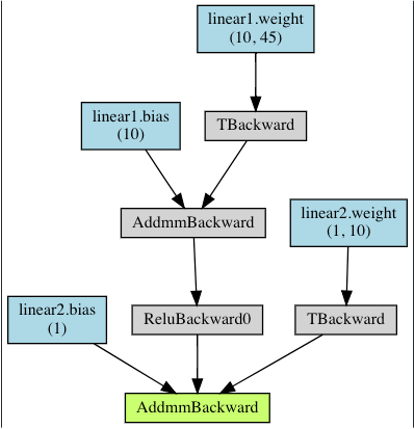
\includegraphics[width=0.5\linewidth]{figures/basic_nn} 

}

\caption{Fig. 1: Architecture of basic neural network used on the similarities of word embeddings.}\label{fig:unnamed-chunk-1}
\end{figure}

In addition to this approach of using word embeddings, I also built a
baseline model using Long Short-Term Memory in Pytorch on the sequences
of words in the transcripts.

Finally, I also used a BERT transformer, but this method performed
poorly.

All code examples that I used as starting points to build these models
can be found commented in my code.

\hypertarget{experiments-results-discussion}{%
\section{5. Experiments/ Results/
Discussion}\label{experiments-results-discussion}}

The main loss function that I used is mean squared error since I am
trying to predict a specific value (as opposed to a discrete prediction
of whether a group of people changed their opinions at all). Below is a
table of the MSEs of the four methods mentioned in section 4.

\begin{longtable}[]{@{}lr@{}}
\toprule
method & MSE\tabularnewline
\midrule
\endhead
One word embedding (spacy) & 0.149\tabularnewline
All word embeddings (spacy) & 0.289\tabularnewline
Basic NN (spacy) & 0.064\tabularnewline
One word eembedding (BERT) & 0.141\tabularnewline
All word embeddings (BERT) & 0.201\tabularnewline
Basic NN (BERT) & 0.152\tabularnewline
LSTM & 0.130\tabularnewline
BERT transformer & 0.227\tabularnewline
\bottomrule
\end{longtable}

Using the word embedding similarity of the 2nd and 10th 1/10th chunks
has a lower loss than using all of the similarities of the embeddings.
But both of these perform worse than a basic neural network.

Despite the varying levels of loss, all of the models seem to be
performing poorly upon closer inspection. If you actually examine the
predicted values, you see that they are all basically the same.
Particularly the basic NN, which has the lowest loss, and the LSTM are
simply finding the best average value and applying that ``prediction''
to all test examples. When I tried to build a more complex neural
network, the problem was only exacerbated. To try to circumvent this
problem, I am going to try to incorporate data from the Priniski paper.

\newpage

\hypertarget{discussion-and-next-steps}{%
\section{6. Discussion and Next Steps}\label{discussion-and-next-steps}}

While the initial goal of training a deep learning model to be able to
identify opinion change was largely unsucessful, there are some key
learnings that I have from this project.

First, I clearly see now that the words that people are using are not
predictive of opinion change. This finding is likely because people talk
about the same things, but they talk about them differently. I came into
this project theorizing that it is not \emph{what} people talk about
that predicts opinion change, it is \emph{how} they talk about it. As
such, my next steps for this project will be to undertake feature
engineering to extract linguistic features, such as polarity,
subjectivity, incivility, and citation of data.

And so, my next steps would be using previously coded examples of
polarizty/ sentiment, incivility, etc. and transformers to build the
features necessary that can be used in a machine or deep learning model
to predict opinion change.

\newpage

\hypertarget{references}{%
\section*{References}\label{references}}
\addcontentsline{toc}{section}{References}

\hypertarget{refs}{}
\leavevmode\hypertarget{ref-fishkin}{}%
Fishkin, James S. 2018. \emph{Democracy When the People Are Thinking:
Revitalizing Our Politics Through Public Deliberation}. Oxford
University Press.

\leavevmode\hypertarget{ref-spacy2}{}%
Honnibal, Matthew, and Ines Montani. 2017. ``spaCy 2: Natural Language
Understanding with Bloom Embeddings, Convolutional Neural Networks and
Incremental Parsing.''

\leavevmode\hypertarget{ref-pytorch}{}%
Paszke, Adam, Sam Gross, Francisco Massa, Adam Lerer, James Bradbury,
Gregory Chanan, Trevor Killeen, et al. 2019. ``PyTorch: An Imperative
Style, High-Performance Deep Learning Library.'' In \emph{Advances in
Neural Information Processing Systems 32}, edited by H. Wallach, H.
Larochelle, A. Beygelzimer, F. Alche-Buc, E. Fox, and R. Garnett,
8024--35. Curran Associates, Inc.
\url{http://papers.neurips.cc/paper/9015-pytorch-an-imperative-style-high-performance-deep-learning-library.pdf}.

\leavevmode\hypertarget{ref-scikit-learn}{}%
Pedregosa, F., G. Varoquaux, A. Gramfort, V. Michel, B. Thirion, O.
Grisel, M. Blondel, et al. 2011. ``Scikit-Learn: Machine Learning in
Python.'' \emph{Journal of Machine Learning Research} 12: 2825--30.

\leavevmode\hypertarget{ref-cmv}{}%
Priniski, John Hunter, and Zach Horne. 2018. ``Attitude Change on
Reddit's Change My View.'' \emph{Conference: Proceedings of the 40th
Annual Meeting of the Cognitive Science Society, Madison, Wisconsin}.
\url{https://www.researchgate.net/publication/333175400_Attitude_Change_on_Reddit's_Change_My_View}.

\leavevmode\hypertarget{ref-zhang}{}%
Zhang, Han, and Jennifer Pan. 2019. ``CASM: A Deep-Learning Approach for
Identifying Collective Action Events with Text and Image Data from
Social Media.'' \emph{Sociological Methodology} 49 (1): 1--57.





\newpage
\singlespacing 
\end{document}
